\documentclass{article} 
\usepackage[shortlabels]{enumitem} 
\usepackage{amsmath}
\usepackage{graphicx}

\begin{document}

\section{Approximation of random walk on time inhomogenous Markov chain}
\begin{figure}
\centering
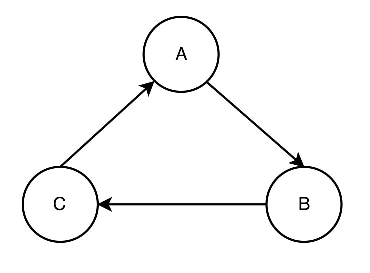
\includegraphics[width=0.5\textwidth]{simple_adjacency}
\caption{Network graph example}
\label{fig:adjacency_1}
\end{figure}

$\mathbf{A}$ is an adjacency matrix of our network which is shown in figure \ref{fig:adjacency_1}.
\[\mathbf{A}=
\begin{bmatrix}
    0 & 0 & 1 \\
    1 & 0 & 0  \\
    0 & 1 & 0 \\
\end{bmatrix}
\]

We can compute transition matrix $\mathbf{P}$ with respect to adjacency matrix $\mathbf{A}$ as a Page Rank transition matrix:
$$\mathbf{P} = \alpha \mathbf{A}\mathbf{D^{-1}} + \frac{1- \alpha}{n} \mathbf{1}\cdot \mathbf{1^T}, $$ where matrix $\mathbf{D}$ is diagonal matrix with elements $D_{ii} = max(k_{i}^{out}, 1)$ where $k_{i}^{out}$ is number of out-degree of each node. Factor $\alpha$ is the probability of following a link from node and $(1 - \alpha)$ is the probability teleporting to any node. Matrix $\mathbf{1}\cdot \mathbf{1^T}$ is square matrix with size $(n\times n)$ where each element is equal to 1.

We want to build hierarchical model in the following way. Suppose we have more than one parameter $\alpha$, which implies that we have more than one transition matrix $\mathbf{P}$. We want to build hierarchical model in the following way: one step is composed of different transition matrix $\mathbf{P_i}$ which is computed with different $\alpha_i$. For the first step we would take $P_1$ with $\alpha_1$, for the second one $P_2$ with $\alpha_2$ and so one. Last $\alpha_i$ is 0. Our hierarchical model with different transition matrices $P_i$ is shown in \ref{fig:adjacency3a}.

\begin{figure}
\centering
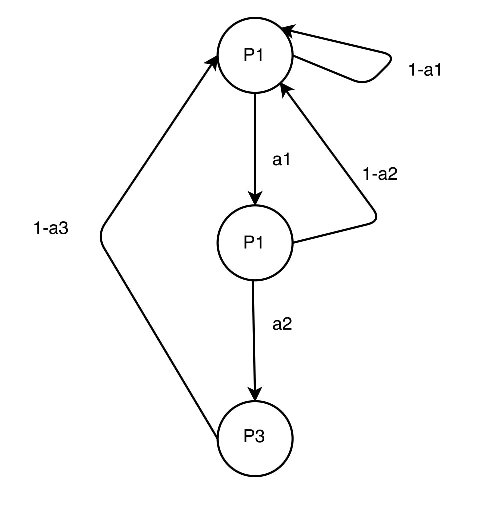
\includegraphics[width=0.5\textwidth]{adjacency3a}
\caption{Hierarchical model}
\label{fig:adjacency3a}
\end{figure}

We can write the transition matrix $\mathbf{P'}$ of the graph \ref{fig:adjacency3a} in the following way:

\[\mathbf{P'}=
\begin{bmatrix}
    1-\alpha_1 & 1-\alpha_2 & 1-\alpha_3  \\
    \alpha_1 & 0 & 0 \\
    0 & \alpha_2 & 0  \\
\end{bmatrix}
\]

We want to compute different transition matrices for our adjacency matrix $\mathbf{A}$ with respect to different parameters $\alpha$: $\mathbf{P_1}$ is transition matrix of $\mathbf{A}$ with parameter $\alpha_1$, $\mathbf{P_2}$ is transition matrix of $\mathbf{A}$ with parameter $\alpha_2$ and $\mathbf{P_3}$ is transition matrix of $\mathbf{A}$ with parameter $\alpha_3$. Our parameters are: $\alpha_1 = 0.8$, $\alpha_2 = 0.4$ and $\alpha_3 = 0$. If we use PageRank formula we get:

\[\mathbf{P_1}=
\begin{bmatrix}
    0.067 &  0.067 &  0.867 \\
    0.867 & 0.067 &  0.067  \\
    0.067 & 0.867 & 0.067 \\
\end{bmatrix}
\]

\[\mathbf{P_2}=
\begin{bmatrix}
    0.2 &  0.2 &  0.6 \\
    0.6 & 0.2 &  0.2  \\
    0.2 & 0.6 & 0.2 \\
\end{bmatrix}
\]

\[\mathbf{P_2}=
\begin{bmatrix}
    0.333 &  0.333 &  0.333 \\
    0.333 & 0.333 &  0.333  \\
    0.333 & 0.333 & 0.333 \\
\end{bmatrix}
\]

 Note that each $\mathbf{P_i}$ matrix is stochastic (sum over the columns is 1).


We can also compute stationary distribution $\mathbf{\pi(P')}$  of the graph $\mathbf{P'}$. We get: 

\begin{equation}
	\mathbf{\pi(P')} = \begin{bmatrix}
	0.47169811 & 0.37735849 & 0.1509434
	\end{bmatrix}
	\label{eq:st_distr_P'_1}
\end{equation}

This tells us the probabilities we will be in the state $\mathbf{P_1}$ (with probability 0.6), $\mathbf{P_2}$  (with probability 0.276) or in $\mathbf{P_3}$ (with probability 0.133). 

We know that $\sum_{i=1}\mathbf{\pi_i} = 1$. Therefore we can combine $\mathbf{\pi}$ and matrices $\mathbf{P_i}$ to get the final transition matrix $\mathbf{P}$:
$$ \mathbf{P} = \mathbf{\pi_1} \cdot \mathbf{P_1} + \mathbf{\pi_2} \cdot \mathbf{P_2} + \mathbf{\pi_3} \cdot \mathbf{P_3}.$$

Applying the results we already computed we get:

\[\mathbf{P}=
\begin{bmatrix}
    0.13777778 &  0.13777778 &  0.72444444 \\
    0.72444444 & 0.13777778 &  0.13777778  \\
    0.13777778 & 0.72444444 & 0.13777778 \\
\end{bmatrix}
\]

Because $\mathbf{P_i}$ are stochastic and $\mathbf{\pi}$ is stationary distribution, matrix $\mathbf{P}$ is also stochastic matrix. Matrix $\mathbf{P}$ tells us with which probabilities we will be in states $A$, $B$ or $C$ (from figure \ref{fig:adjacency_1}) if we dynamically change probabilities $\alpha_i$ and randomly walk on graph \ref{fig:adjacency3a}. 

We will calculate stationary distribution $\mathbf{\pi(P)}$ of matrix $\mathbf{P}$ as well:

\begin{equation}
	\mathbf{\pi(P)} = \begin{bmatrix}
	0.33333333 & 0.33333333 & 0.33333333
	\end{bmatrix}
	\label{eq:st_distr_P_1}
\end{equation}


\section{Exact solution of random walk on time inhomogenous Markov chain}

In this part we have to write all the states that are possible if we take into account our two graphs on figures \ref{fig:adjacency3a}, \ref{fig:adjacency_1}. We have 3 states from graph \ref{fig:adjacency_1} and 3 states from graph \ref{fig:adjacency3a}, which are actually time states. Altogether we have 9 states which are denoted as: $A1, B1, C1, A2, B2, C2, A3, B3, C3$. States $A1, B1, C1$ actually represents graph \ref{fig:adjacency_1} in state $P_1$ from graph \ref{fig:adjacency3a} with probability $\alpha_1$. Also, same applies for all other states.

\begin{figure}
\centering
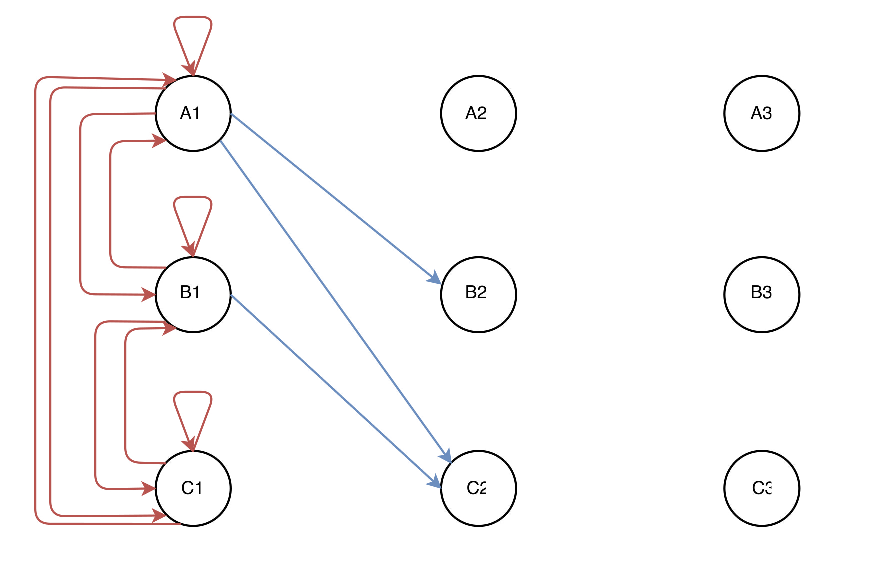
\includegraphics[width=0.5\textwidth]{tihMC_1_step}
\caption{Transitions for the first time step}
\label{fig:tihMC_1_step}
\end{figure}

We can draw the transitions between these states ($Ai, Bi, Ci$). For the first time step, transitions are shown in figure \ref{fig:tihMC_1_step}. Blue arrows represents random surfer decision to follow links with probability $\frac{\alpha_1}{k_{out}}$. The direction is determined by graph in figure \ref{fig:adjacency_1}. Red arrows represent probability of jumping to any node in first time step: $\frac{1-\alpha_1}{3}$.


\begin{figure}
\centering
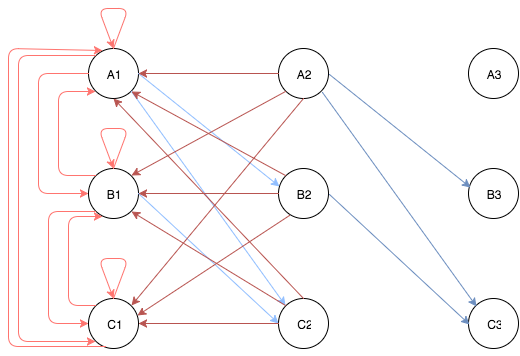
\includegraphics[width=0.5\textwidth]{tihMC_2_step}
\caption{Transitions for the second time step}
\label{fig:tihMC_2_step}
\end{figure}

Second time step is in figure \ref{fig:tihMC_2_step}. Again, blue arrows represents the random surfer decision to follow links, probability is similar as before:  $\frac{\alpha_2}{k_{out}}$. Red arrows again represents probability of teleportation. The direction of teleportation is determined by the graph in figure \ref{fig:adjacency3a} (we are always jumping back to the first time step). Probabilities are similar as before: $\frac{1-\alpha_2}{3}$.


\begin{figure}
\centering
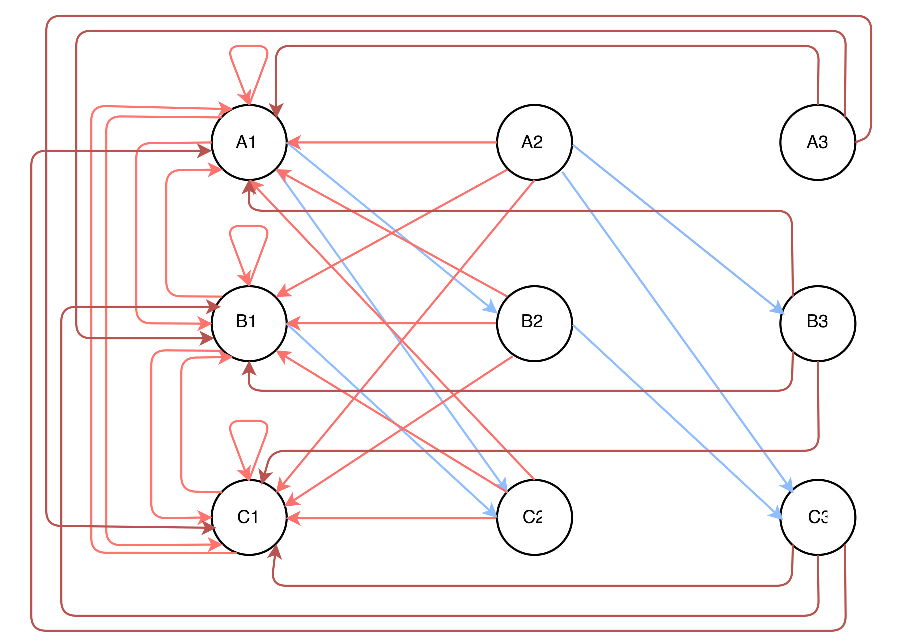
\includegraphics[width=0.5\textwidth]{tihMC_3_step}
\caption{Transitions for the last time step}
\label{fig:tihMC_3_step}
\end{figure}

Last step consists of only teleportations back to the first time step and is shown in figure \ref{fig:tihMC_3_step}. The probabilities of jumping back are $\frac{1-\alpha_3}{3} = \frac{1}{3}$.

We can finally write our transition matrix $\mathbf{T}$ for this example:

\[\mathbf{T}=
\begin{bmatrix}
    \frac{1-\alpha_1}{3} &  \frac{1-\alpha_2}{3} & \frac{1-\alpha_3}{3} & \frac{1-\alpha_1}{3} &  \frac{1-\alpha_2}{3} & \frac{1-\alpha_3}{3} & \frac{1-\alpha_1}{3} &  \frac{1-\alpha_2}{3} & \frac{1-\alpha_3}{3} \\
    0 & 0 & 0 & 0 & 0 & 0 & \alpha_1 & 0 & 0 \\
    0 & 0 & 0 & 0 & 0 & 0 & 0 & \alpha_2 & 0 \\
        \frac{1-\alpha_1}{3} &  \frac{1-\alpha_2}{3} & \frac{1-\alpha_3}{3} & \frac{1-\alpha_1}{3} &  \frac{1-\alpha_2}{3} & \frac{1-\alpha_3}{3} & \frac{1-\alpha_1}{3} &  \frac{1-\alpha_2}{3} & \frac{1-\alpha_3}{3} \\
	    \alpha_1 & 0 & 0 & 0 & 0 & 0 & 0 & 0 & 0 \\
	   0 & \alpha_2 & 0 & 0 & 0 & 0 & 0 & 0 & 0 \\
        \frac{1-\alpha_1}{3} &  \frac{1-\alpha_2}{3} & \frac{1-\alpha_3}{3} & \frac{1-\alpha_1}{3} &  \frac{1-\alpha_2}{3} & \frac{1-\alpha_3}{3} & \frac{1-\alpha_1}{3} &  \frac{1-\alpha_2}{3} & \frac{1-\alpha_3}{3} \\
		  0 & 0 & 0 & \alpha_1 & 0 & 0 & 0 & 0 & 0 \\
		  0 & 0 & 0 & 0 & \alpha_2 & 0 & 0 & 0 & 0 \\

\end{bmatrix}
\]


\[\mathbf{T}=
\begin{bmatrix}
    0.06666667 & 0.2 & 0.33333333 &  0.06666667 &  0.2 & 0.33333333 & 0.06666667 & 0.2 & 0.33333333 \\
    0 & 0 & 0 & 0 & 0 & 0 & 0.8 & 0 & 0 \\
    0 & 0 & 0 & 0 & 0 & 0 & 0 & 0.4 & 0 \\
       0.06666667 & 0.2 & 0.33333333 &  0.06666667 &  0.2 & 0.33333333 & 0.06666667 & 0.2 & 0.33333333 \\
	   0.8 & 0 & 0 & 0 & 0 & 0 & 0 & 0 & 0 \\
	   0 & 0.4 & 0 & 0 & 0 & 0 & 0 & 0 & 0 \\
       0.06666667 & 0.2 & 0.33333333 &  0.06666667 &  0.2 & 0.33333333 & 0.06666667 & 0.2 & 0.33333333 \\
		  0 & 0 & 0 & 0.8 & 0 & 0 & 0 & 0 & 0 \\
		  0 & 0 & 0 & 0 &0.4 & 0 & 0 & 0 & 0 \\

\end{bmatrix}
\]

We can calculate stationary distribution of matrix $\mathbf{T}$:
\[\mathbf{\pi(T)} = 
\begin{bmatrix}
0.15723  & 0.125786 &  0.050314&  0.15723  & 0.125786 &  0.050314&  0.15723 &  0.125786 & 0.050314 \\
\end{bmatrix}
\]


Stationary distribution $\mathbf{\pi_T}$ of matrix $\mathbf{T}$ tells us, that we will be in state $A1$ with probability $0.1572327$, in state $A2$ with probability $0.18867925$, in state $A3$ with probability $0.05031447$ and so on. States $A1, B1, C1$ can be represented as matrix $\mathbf{P_1}$ with probability $\alpha_1$ (what we already have calculated in previous section), states $A2, B2, C2$ can be represented with matrix $\mathbf{P_2}$ and lastly, states $A3, B3, C3$ can be represented with matrix $\mathbf{P_3}$. 

We can therefore write our stationary distribution in such a way, that we merge the states that are under same matrix $P_i$, meaning: 
\[\mathbf{\pi(P'*)} = 
\begin{bmatrix}
\pi(P_1) & \pi(P_2) & \pi(P_3) \\
\end{bmatrix}
= \begin{bmatrix}
\pi(A1+B1+C1) & \pi(A2 + B2+C2) & \pi(A3 + B3 + C3) \\
\end{bmatrix}
\]

\[\mathbf{\pi(P'*)} = \begin{bmatrix}
	0.471698113208 & 0.377358490566 & 0.150943396226
	\end{bmatrix}
\]

We can see that we get the same results as in equation \ref{eq:st_distr_P'_1} in the previous section.

We can also sum up stationary distributions of nodes:
\[\mathbf{\pi(P*)} = 
\begin{bmatrix}
\pi(A1+A2+A3), \pi(B1+B2+B3), \pi(C1+C2+C3) \\
\end{bmatrix}
\]

\[\mathbf{\pi(P*)} = 
\begin{bmatrix}
0.33 & 0.33 & 0.33 \\
\end{bmatrix}
\]

We can see that computed stationary distribution is the same as the stationary distribution $\pi(P)$ in equation \ref{eq:st_distr_P_1}.

\section{More examples}
The first network example in figure \ref{fig:adjacency_1} was really simple. Lets take a look at more complex examples. Note that the probabilities are the same as before.

\subsection{First example}

\begin{figure}
\centering
\includegraphics[width=0.5\textwidth]{adj2}
\caption{Network graph example}
\label{fig:adj2}
\end{figure}
The network is illustrated in figure \ref{fig:adj2}. We can write adjacency matrix $\mathbf{A}$ for this example:
\[\mathbf{A} = 
\begin{bmatrix}
0  & 1  & 1 \\
1 & 0 & 0 \\
0 & 1 & 0\\
\end{bmatrix}
\]

We will use same transition matrix $\mathbf{P'}$ (in figure \ref{fig:adjacency3a}). Therefore the stationary distribution of this transition matrix $\mathbf{P'}$ is the same as in previous example:
\begin{equation}
\mathbf{\pi(P')} = \begin{bmatrix}
	0.47169811 &  0.37735849 & 0.1509434\\
	\end{bmatrix}
	\label{eq:st_distr_P'_2}
\end{equation}

However the network is not the same as before, therefore our transition matrix $\mathbf{T}$ will be different.

\[\mathbf{T}=
\begin{bmatrix}
    \frac{1-\alpha_1}{3} &  \frac{1-\alpha_2}{3} & \frac{1-\alpha_3}{3} & \frac{1-\alpha_1}{3} &  \frac{1-\alpha_2}{3} & \frac{1-\alpha_3}{3} & \frac{1-\alpha_1}{3} &  \frac{1-\alpha_2}{3} & \frac{1-\alpha_3}{3} \\
    0 & 0 & 0 &  \frac{\alpha_1}{2} & 0 & 0 & \alpha_1 & 0 & 0 \\
    0 & 0 & 0 & 0 & \frac{\alpha_2}{2} & 0 & 0 & \alpha_2 & 0 \\
        \frac{1-\alpha_1}{3} &  \frac{1-\alpha_2}{3} & \frac{1-\alpha_3}{3} & \frac{1-\alpha_1}{3} &  \frac{1-\alpha_2}{3} & \frac{1-\alpha_3}{3} & \frac{1-\alpha_1}{3} &  \frac{1-\alpha_2}{3} & \frac{1-\alpha_3}{3} \\
	    \alpha_1 & 0 & 0 & 0 & 0 & 0 & 0 & 0 & 0 \\
	   0 & \alpha_2 & 0 & 0 & 0 & 0 & 0 & 0 & 0 \\
        \frac{1-\alpha_1}{3} &  \frac{1-\alpha_2}{3} & \frac{1-\alpha_3}{3} & \frac{1-\alpha_1}{3} &  \frac{1-\alpha_2}{3} & \frac{1-\alpha_3}{3} & \frac{1-\alpha_1}{3} &  \frac{1-\alpha_2}{3} & \frac{1-\alpha_3}{3} \\
		  0 & 0 & 0 & \frac{\alpha_1}{2} & 0 & 0 & 0 & 0 & 0 \\
		  0 & 0 & 0 & 0 & \frac{\alpha_2}{2} & 0 & 0 & 0 & 0 \\

\end{bmatrix}
\]

Plugging in the values, we get:

\[\mathbf{T}=
\begin{bmatrix}
    0.06666667 & 0.2 & 0.33333333 &  0.06666667 &  0.2 & 0.33333333 & 0.06666667 & 0.2 & 0.33333333 \\
    0 & 0 & 0 & 0.4 & 0 & 0 & 0.8 & 0 & 0 \\
    0 & 0 & 0 & 0 & 0.2 & 0 & 0 & 0.4 & 0 \\
       0.06666667 & 0.2 & 0.33333333 &  0.06666667 &  0.2 & 0.33333333 & 0.06666667 & 0.2 & 0.33333333 \\
	   0.8 & 0 & 0 & 0 & 0 & 0 & 0 & 0 & 0 \\
	   0 & 0.4 & 0 & 0 & 0 & 0 & 0 & 0 & 0 \\
       0.06666667 & 0.2 & 0.33333333 &  0.06666667 &  0.2 & 0.33333333 & 0.06666667 & 0.2 & 0.33333333 \\
		  0 & 0 & 0 & 0.4 & 0 & 0 & 0 & 0 & 0 \\
		  0 & 0 & 0 & 0 &0.2 & 0 & 0 & 0 & 0 \\

\end{bmatrix}
\]

Stationary distribution $\mathbf{\pi(T)}$ of matrix $\mathbf{T}$ is:
\[\mathbf{\pi(T)} = \begin{bmatrix}
	0.15723 & 0.188679 & 0.050314 & 0.15723 &  0.125786 & 0.07547 & 0.15723 &  0.062893 & 0.025157\\
	\end{bmatrix}
\]


Again, we can sum up nodes which are generated under the same probability:                   
\[\mathbf{\pi(P'*)} = 
\begin{bmatrix}
\pi(P_1) & \pi(P_2) & \pi(P_3) \\
\end{bmatrix}
= \begin{bmatrix}
\pi(A1+B1+C1) & \pi(A2 + B2+C2) & \pi(A3 + B3 + C3) \\
\end{bmatrix}
\]
\[\mathbf{\pi(P'*)} = 
\begin{bmatrix}
0.471698113208 & 0.377358490566 & 0.150943396226 \\
\end{bmatrix}
\]

We can see that stationary distribution is again the same as stationary distribution of transition matrix $\mathbf{P'}$ (equation \ref{eq:st_distr_P'_2}.

We can also sum up stationary distribution by nodes (A1+A2+A3) etc.:
\[\mathbf{\pi} = 
\begin{bmatrix}
\pi(A1+A2+A3), \pi(B1+B2+B3), \pi(C1+C2+C3) \\
\end{bmatrix}
\]

\begin{equation}
\mathbf{\pi(P*)} = 
\begin{bmatrix}
0.396226415094 & 0.358490566038 & 0.245283018868 \\
\end{bmatrix}
\label{eq:st_distr_P_2_*}
\end{equation}

In order to verify the result from equation \ref{eq:st_distr_P_2_*}, we have to compute matrix $\mathbf{P}$ and its stationary distribution.


\[\mathbf{P}=
\begin{bmatrix}
    0.13777778 &  0.43111111 &  0.72444444 \\
    0.72444444 & 0.13777778 & 0.13777778  \\
    0.13777778 & 0.43111111 & 0.13777778 \\
\end{bmatrix}
\]


Stationary distribution $\pi(P)$ of matrix $P$ is:
\begin{equation}
\mathbf{\pi(P)} = 
\begin{bmatrix}
0.38612593 &  0.36122376 & 0.2526503
\end{bmatrix}
\label{eq:st_distr_P_2}
\end{equation}

The results from equations \ref{eq:st_distr_P_2} and \ref{eq:st_distr_P_2_*} are almost the same.

\subsection{Second example (?) To think about it}
Second example is in figure  \ref{fig:adj_2}. Note that node C does not have any outlinks. 
\begin{figure}
\centering
\includegraphics[width=0.5\textwidth]{adj_2}
\caption{Network graph example}
\label{fig:adj_2}
\end{figure}

We can write adjacency matrix \textbf{A}:
\[\mathbf{A} = 
\begin{bmatrix}
0  & 0  & 0 \\
1 & 0 & 0 \\
1 & 1 & 0\\
\end{bmatrix}
\]

Again, we will use the same transition matrix \textbf{P'} (figure \ref{fig:adjacency3a}) and the stationary distribution is the same: 
\[\mathbf{\pi(P')} = \begin{bmatrix}
	0.47169811 &  0.37735849 & 0.1509434\\
	\end{bmatrix}
\]

The transition matrix $\mathbf{T}$ is different:


\[\mathbf{T}=
\begin{bmatrix}
    \frac{1-\alpha_1}{3} &  \frac{1-\alpha_2}{3} & \frac{1-\alpha_3}{3} & \frac{1-\alpha_1}{3} &  \frac{1-\alpha_2}{3} & \frac{1-\alpha_3}{3} & \frac{1-\alpha_1}{3} &  \frac{1-\alpha_2}{3} & \frac{1-\alpha_3}{3} \\
    0 & 0 & 0 &  0 & 0 & 0 & 0 & 0 & 0 \\
    0 & 0 & 0 & 0 & 0 & 0 & 0 & 0 & 0 \\
        \frac{1-\alpha_1}{3} &  \frac{1-\alpha_2}{3} & \frac{1-\alpha_3}{3} & \frac{1-\alpha_1}{3} &  \frac{1-\alpha_2}{3} & \frac{1-\alpha_3}{3} & \frac{1-\alpha_1}{3} &  \frac{1-\alpha_2}{3} & \frac{1-\alpha_3}{3} \\
	    \frac{\alpha_1}{2} & 0 & 0 & 0 & 0 & 0 & 0 & 0 & 0 \\
	   0 & \frac{\alpha_2}{2} & 0 & 0 & 0 & 0 & 0 & 0 & 0 \\
        \frac{1-\alpha_1}{3} &  \frac{1-\alpha_2}{3} & \frac{1-\alpha_3}{3} & \frac{1-\alpha_1}{3} &  \frac{1-\alpha_2}{3} & \frac{1-\alpha_3}{3} & \frac{1-\alpha_1}{3} &  \frac{1-\alpha_2}{3} & \frac{1-\alpha_3}{3} \\
		   \frac{\alpha_1}{2} & 0 & 0 & \alpha_1 & 0 & 0 & 0 & 0 & 0 \\
		  0 & \frac{\alpha_2}{2} & 0 & 0 & \alpha_2 & 0 & 0 & 0 & 0 \\

\end{bmatrix}
\]


\[\mathbf{T}=
\begin{bmatrix}
    0.06666667 & 0.2 & 0.33333333 &  0.06666667 &  0.2 & 0.33333333 & 0.06666667 & 0.2 & 0.33333333 \\
    0 & 0 & 0 & 0 & 0 & 0 & 0 & 0 & 0 \\
    0 & 0 & 0 & 0 & 0 & 0 & 0 & 0 & 0 \\
       0.06666667 & 0.2 & 0.33333333 &  0.06666667 &  0.2 & 0.33333333 & 0.06666667 & 0.2 & 0.33333333 \\
	   0.4 & 0 & 0 & 0 & 0 & 0 & 0 & 0 & 0 \\
	   0 & 0.2 & 0 & 0 & 0 & 0 & 0 & 0 & 0 \\
       0.06666667 & 0.2 & 0.33333333 &  0.06666667 &  0.2 & 0.33333333 & 0.06666667 & 0.2 & 0.33333333 \\
		  0.4 & 0 & 0 & 0.8 & 0 & 0 & 0 & 0 & 0 \\
		  0 & 0.2 & 0 & 0 &0.4 & 0 & 0 & 0 & 0 \\

\end{bmatrix}
\]

Note that matrix $\mathbf{T}$ is not really stochastic (7th and 8th column do not sum up to 1 because  C does not have any outgoing links).

Stationary distribution of the matrix $\mathbf{T}$ is:
\[\mathbf{\pi} = \begin{bmatrix}
	0.23076923 & 0. &  0. & 0.23076923 &  0.05128205 &  0.02564103 &  0.23076923 & 0.15384615 & 0.07692308\\
	\end{bmatrix}
\]

Again, we can sum up nodes which are generated under the same probability:                   
\[\mathbf{\pi} = 
\begin{bmatrix}
\pi(P_1) & \pi(P_2) & \pi(P_3) \\
\end{bmatrix}
= \begin{bmatrix}
\pi(A1+B1+C1) & \pi(A2 + B2+C2) & \pi(A3 + B3 + C3) \\
\end{bmatrix}
\]
\[\mathbf{\pi} = 
\begin{bmatrix}
0.692307692308 & 0.205128205128 & 0.102564102564\\
\end{bmatrix}
\]

The probabilities are almost the same as the stationary distribution of $\mathbf{P'}$.


We can also sum up stationary distribution by nodes (A1+A2+A3) etc.:
\[\mathbf{\pi} = 
\begin{bmatrix}
\pi(A1+A2+A3), \pi(B1+B2+B3), \pi(C1+C2+C3) \\
\end{bmatrix}
\]


\begin{equation}
\mathbf{\pi} = 
\begin{bmatrix}
0.230769230769 & 0.307692307692 & 0.461538461538 \\
\end{bmatrix}
\label{eq:2_ex}
\end{equation}


In order to verify the result from equation \ref{eq:2_ex}, we have to compute matrix $\mathbf{P}$ and its stationary distribution.

\[\mathbf{P}=
\begin{bmatrix}
    0.13777778 &  0.13777778 &  0.33333333 \\
    0.43111111 & 0.13777778 & 0.33333333  \\
    0.43111111 & 0.72444444 & 0.33333333 \\
\end{bmatrix}
\]

Corresponding stationary distribution of matrix $\mathbf{P}$:
\begin{equation}
[\mathbf{\pi(P)} = 
\begin{bmatrix}
0.2383134 & 0.3012641 & 0.4604225
\end{bmatrix}
\label{eq:2_ex_v}
\end{equation}


\section{Generating transition matrix T}
Before we actually write down the transition matrix $\mathbf{T}$. However it is possible to generate it from adjacency matrix $\mathbf{A}$ and transition matrix $\mathbf{P'}$. Note that for now it only works for such adjacency matrices that each node in that matrix has at least one outgoing link. 

In order to generate matrix $\mathbf{T}$, we have to first "normalize" adjacency matrix $\mathbf{A}$ (to take care of the nodes that have more than one outgoing link). Then we calculate the Kronecker product of $\mathbf{A_{norm}}$ and $\mathbf{P'}$:

$$\mathbf{T'} = \mathbf{A_{norm}} \otimes \mathbf{P'}.$$

Also we know that the first (0-th) row, and all i-th rows that are by modulo of number of transition probabilities $\alpha$ 0, contains only teleportation probabilities. We can replace those rows by teleportation probabilities and this is already our matrix $\mathbf{T}$.  

In order to verify our method, we calculate the stationary distribution of matrix $\mathbf{T}$ and sum it up in two ways as before (one way: group all same nodes from $\mathbf{A}$ together, another way: group all nodes from $\mathbf{P'}$ together) and compare it to stationary distributions of $\mathbf{P'}$ and $\mathbf{P}$.

This method works (there are around 1\% deviations in simple examples, which could be due to numeric precision). 


\end{document}